% Options for packages loaded elsewhere
% Options for packages loaded elsewhere
\PassOptionsToPackage{unicode}{hyperref}
\PassOptionsToPackage{hyphens}{url}
%
\documentclass[
  ignorenonframetext,
  aspectratio=169,
  russian,
]{beamer}
\newif\ifbibliography
\usepackage{pgfpages}
\setbeamertemplate{caption}[numbered]
\setbeamertemplate{caption label separator}{: }
\setbeamercolor{caption name}{fg=normal text.fg}
\beamertemplatenavigationsymbolshorizontal
% remove section numbering
\setbeamertemplate{part page}{
  \centering
  \begin{beamercolorbox}[sep=16pt,center]{part title}
    \usebeamerfont{part title}\insertpart\par
  \end{beamercolorbox}
}
\setbeamertemplate{section page}{
  \centering
  \begin{beamercolorbox}[sep=12pt,center]{section title}
    \usebeamerfont{section title}\insertsection\par
  \end{beamercolorbox}
}
\setbeamertemplate{subsection page}{
  \centering
  \begin{beamercolorbox}[sep=8pt,center]{subsection title}
    \usebeamerfont{subsection title}\insertsubsection\par
  \end{beamercolorbox}
}
% Prevent slide breaks in the middle of a paragraph
\widowpenalties 1 10000
\raggedbottom
\AtBeginPart{
  \frame{\partpage}
}
\AtBeginSection{
  \ifbibliography
  \else
    \frame{\sectionpage}
  \fi
}
\AtBeginSubsection{
  \frame{\subsectionpage}
}
\usepackage{iftex}
\ifPDFTeX
  \usepackage[T1]{fontenc}
  \usepackage[utf8]{inputenc}
  \usepackage{textcomp} % provide euro and other symbols
\else % if luatex or xetex
  \usepackage{unicode-math} % this also loads fontspec
  \defaultfontfeatures{Scale=MatchLowercase}
  \defaultfontfeatures[\rmfamily]{Ligatures=TeX,Scale=1}
\fi
\usepackage{lmodern}

\ifPDFTeX\else
  % xetex/luatex font selection
\fi
% Use upquote if available, for straight quotes in verbatim environments
\IfFileExists{upquote.sty}{\usepackage{upquote}}{}
\IfFileExists{microtype.sty}{% use microtype if available
  \usepackage[]{microtype}
  \UseMicrotypeSet[protrusion]{basicmath} % disable protrusion for tt fonts
}{}


\usepackage{longtable,booktabs,array}
\usepackage{calc} % for calculating minipage widths
\usepackage{caption}
% Make caption package work with longtable
\makeatletter
\def\fnum@table{\tablename~\thetable}
\makeatother
\usepackage{graphicx}
\makeatletter
\newsavebox\pandoc@box
\newcommand*\pandocbounded[1]{% scales image to fit in text height/width
  \sbox\pandoc@box{#1}%
  \Gscale@div\@tempa{\textheight}{\dimexpr\ht\pandoc@box+\dp\pandoc@box\relax}%
  \Gscale@div\@tempb{\linewidth}{\wd\pandoc@box}%
  \ifdim\@tempb\p@<\@tempa\p@\let\@tempa\@tempb\fi% select the smaller of both
  \ifdim\@tempa\p@<\p@\scalebox{\@tempa}{\usebox\pandoc@box}%
  \else\usebox{\pandoc@box}%
  \fi%
}
% Set default figure placement to htbp
\def\fps@figure{htbp}
\makeatother



\ifLuaTeX
\usepackage[bidi=basic,provide=*]{babel}
\else
\usepackage[bidi=default,provide=*]{babel}
\fi
% get rid of language-specific shorthands (see #6817):
\let\LanguageShortHands\languageshorthands
\def\languageshorthands#1{}


\setlength{\emergencystretch}{3em} % prevent overfull lines

\providecommand{\tightlist}{%
  \setlength{\itemsep}{0pt}\setlength{\parskip}{0pt}}



 

\usepackage[]{csquotes}

\IfFileExists{plex-otf.sty}{
  %% Full TeXlive
  % \usepackage[%
  %   % math,
  %   RM={Scale=0.94},SS={Scale=0.94},SScon={Scale=0.94},TT={Scale=MatchLowercase,FakeStretch=0.9},DefaultFeatures={Ligatures=Common}
  % ]{plex-otf}
}{
  %% TinyTeX
  \usepackage{libertine}
}

%%% Load theme
% https://deic.uab.cat/~iblanes/beamer_gallery/
\IfFileExists{beamerthemegotham.sty}{
  %% Full TeXlive
  \usetheme{gotham}
  \gothamset{
    numbering=totalpagenumber,
    parttocframe default=off,
    sectiontocframe default=off,
    subsectiontocframe default=off,
  }
}{
  %% TinyTeX
  \usetheme{Madrid}
}
\makeatletter
\@ifpackageloaded{caption}{}{\usepackage{caption}}
\AtBeginDocument{%
\ifdefined\contentsname
  \renewcommand*\contentsname{Содержание}
\else
  \newcommand\contentsname{Содержание}
\fi
\ifdefined\listfigurename
  \renewcommand*\listfigurename{Список иллюстраций}
\else
  \newcommand\listfigurename{Список иллюстраций}
\fi
\ifdefined\listtablename
  \renewcommand*\listtablename{Список таблиц}
\else
  \newcommand\listtablename{Список таблиц}
\fi
\ifdefined\figurename
  \renewcommand*\figurename{Рисунок}
\else
  \newcommand\figurename{Рисунок}
\fi
\ifdefined\tablename
  \renewcommand*\tablename{Таблица}
\else
  \newcommand\tablename{Таблица}
\fi
}
\@ifpackageloaded{float}{}{\usepackage{float}}
\floatstyle{ruled}
\@ifundefined{c@chapter}{\newfloat{codelisting}{h}{lop}}{\newfloat{codelisting}{h}{lop}[chapter]}
\floatname{codelisting}{Список}
\newcommand*\listoflistings{\listof{codelisting}{Листинги}}
\makeatother
\makeatletter
\makeatother
\makeatletter
\@ifpackageloaded{caption}{}{\usepackage{caption}}
\@ifpackageloaded{subcaption}{}{\usepackage{subcaption}}
\makeatother

\usepackage{bookmark}
\IfFileExists{xurl.sty}{\usepackage{xurl}}{} % add URL line breaks if available
\urlstyle{same}
\hypersetup{
  pdftitle={Лабораторная работа № 4},
  pdflang={ru-RU},
  hidelinks,
  pdfcreator={LaTeX via pandoc}}


\title{Лабораторная работа № 4}
\subtitle{Дискреционное разграничение прав в Linux. Расширенные
атрибуты}
\author{Прядко Алексей Семенович}
\date{2026-04-04}

\begin{document}
\frame{\titlepage}

\renewcommand*\contentsname{Содержание}
\begin{frame}[allowframebreaks]
  \frametitle{Содержание}
  \setcounter{tocdepth}{1}
  \tableofcontents
\end{frame}
\setcounter{tocdepth}{1}
\tableofcontents
}

\section{Информация}\label{ux438ux43dux444ux43eux440ux43cux430ux446ux438ux44f}

\begin{frame}{Докладчик}
\phantomsection\label{ux434ux43eux43aux43bux430ux434ux447ux438ux43a}
\begin{itemize}[<+->]
\tightlist
\item
  {[}Прядко Алексей Семенович{]}
\item
  Российский университет дружбы народов
\end{itemize}
\end{frame}

\section{Вводная
часть}\label{ux432ux432ux43eux434ux43dux430ux44f-ux447ux430ux441ux442ux44c}

\begin{frame}[fragile]{Актуальность}
\phantomsection\label{ux430ux43aux442ux443ux430ux43bux44cux43dux43eux441ux442ux44c}
\begin{itemize}[<+->]
\tightlist
\item
  Стандартных дискреционных прав (чтение, запись, выполнение) не всегда
  достаточно.
\item
  Владелец файла может случайно удалить или испортить важные данные.
\item
  Расширенные атрибуты (такие как \texttt{a} и \texttt{i}) позволяют
  создать дополнительный уровень защиты на уровне файловой системы.
\item
  Управлять данными атрибутами имеет право только администратор системы.
\end{itemize}
\end{frame}

\begin{frame}[fragile]{Цели и задачи}
\phantomsection\label{ux446ux435ux43bux438-ux438-ux437ux430ux434ux430ux447ux438}
\textbf{Цель:} Получение практических навыков работы в консоли ОС Linux
с расширенными атрибутами файлов.

\textbf{Задачи:}

\begin{enumerate}[<+->]
\tightlist
\item
  Изучить работу утилит \texttt{lsattr} и \texttt{chattr}.
\item
  Проверить механизм защиты с помощью атрибута \texttt{a} (append-only).
\item
  Проверить механизм абсолютной блокировки с помощью атрибута \texttt{i}
  (immutable).
\end{enumerate}
\end{frame}

\section{Выполнение лабораторной
работы}\label{ux432ux44bux43fux43eux43bux43dux435ux43dux438ux435-ux43bux430ux431ux43eux440ux430ux442ux43eux440ux43dux43eux439-ux440ux430ux431ux43eux442ux44b}

\begin{frame}[fragile]{Базовые права и атрибуты}
\phantomsection\label{ux431ux430ux437ux43eux432ux44bux435-ux43fux440ux430ux432ux430-ux438-ux430ux442ux440ux438ux431ux443ux442ux44b}
\begin{itemize}[<+->]
\tightlist
\item
  С помощью команды \texttt{lsattr} проверены текущие расширенные
  атрибуты тестового файла.
\item
  Командой \texttt{chmod\ 600} установлены права на чтение и запись
  только для владельца.
\end{itemize}

\begin{figure}[H]

{\centering 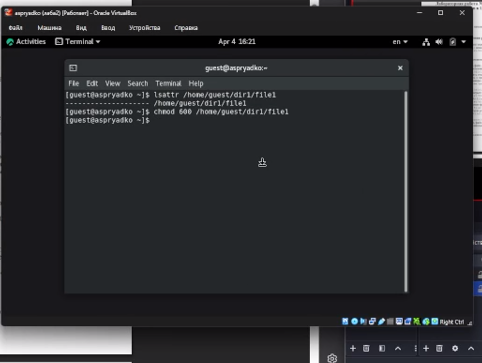
\includegraphics[width=0.6\linewidth,height=\textheight,keepaspectratio]{image/01_base.png}

}

\caption{Установка базовых прав}

\end{figure}%
\end{frame}

\begin{frame}[fragile]{Попытка управления от обычного пользователя}
\phantomsection\label{ux43fux43eux43fux44bux442ux43aux430-ux443ux43fux440ux430ux432ux43bux435ux43dux438ux44f-ux43eux442-ux43eux431ux44bux447ux43dux43eux433ux43e-ux43fux43eux43bux44cux437ux43eux432ux430ux442ux435ux43bux44f}
\begin{itemize}[<+->]
\tightlist
\item
  Обычный пользователь (\texttt{guest}) попытался установить расширенный
  атрибут.
\item
  Система заблокировала действие (Operation not permitted).
\end{itemize}

\begin{figure}[H]

{\centering 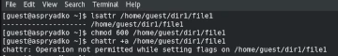
\includegraphics[width=0.6\linewidth,height=\textheight,keepaspectratio]{image/02_guest_fail.png}

}

\caption{Ошибка установки атрибута пользователем}

\end{figure}%
\end{frame}

\begin{frame}[fragile]{Установка атрибута \enquote{a}
суперпользователем}
\phantomsection\label{ux443ux441ux442ux430ux43dux43eux432ux43aux430-ux430ux442ux440ux438ux431ux443ux442ux430-a-ux441ux443ux43fux435ux440ux43fux43eux43bux44cux437ux43eux432ux430ux442ux435ux43bux435ux43c}
\begin{itemize}[<+->]
\tightlist
\item
  Права повышены до администратора (\texttt{su\ -}).
\item
  Успешно установлен атрибут \texttt{a} (append-only) с помощью команды
  \texttt{chattr\ +a}.
\end{itemize}

\begin{figure}[H]

{\centering 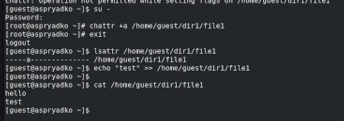
\includegraphics[width=0.6\linewidth,height=\textheight,keepaspectratio]{image/03_root_a.png}

}

\caption{Проверка наличия атрибута \enquote{a}}

\end{figure}%
\end{frame}

\begin{frame}[fragile]{Проверка разрешенных действий (дозапись)}
\phantomsection\label{ux43fux440ux43eux432ux435ux440ux43aux430-ux440ux430ux437ux440ux435ux448ux435ux43dux43dux44bux445-ux434ux435ux439ux441ux442ux432ux438ux439-ux434ux43eux437ux430ux43fux438ux441ux44c}
\begin{itemize}[<+->]
\tightlist
\item
  Атрибут \texttt{a} разрешает исключительно добавление информации в
  конец файла.
\item
  Команда \texttt{echo\ "test"\ \textgreater{}\textgreater{}\ file1}
  выполнилась успешно.
\end{itemize}

\begin{figure}[H]

{\centering 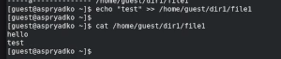
\includegraphics[width=0.6\linewidth,height=\textheight,keepaspectratio]{image/04_append.png}

}

\caption{Успешная дозапись в файл}

\end{figure}%
\end{frame}

\begin{frame}[fragile]{Проверка запрещенных действий}
\phantomsection\label{ux43fux440ux43eux432ux435ux440ux43aux430-ux437ux430ux43fux440ux435ux449ux435ux43dux43dux44bux445-ux434ux435ux439ux441ux442ux432ux438ux439}
\begin{itemize}[<+->]
\tightlist
\item
  Атрибут \texttt{a} блокирует удаление (\texttt{rm}), переименование
  (\texttt{mv}), перезапись (\texttt{\textgreater{}}) и изменение
  базовых прав доступа.
\item
  Все попытки выполнить эти действия завершились ошибкой доступа.
\end{itemize}

\begin{figure}[H]

{\centering 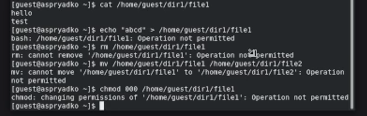
\includegraphics[width=0.6\linewidth,height=\textheight,keepaspectratio]{image/05_denied.png}

}

\caption{Блокировка запрещенных операций}

\end{figure}%
\end{frame}

\begin{frame}[fragile]{Снятие расширенного атрибута}
\phantomsection\label{ux441ux43dux44fux442ux438ux435-ux440ux430ux441ux448ux438ux440ux435ux43dux43dux43eux433ux43e-ux430ux442ux440ux438ux431ux443ux442ux430}
\begin{itemize}[<+->]
\tightlist
\item
  Администратор снял защиту командой \texttt{chattr\ -a}.
\item
  После этого файл снова стал доступен для перезаписи и изменения прав
  (\texttt{chmod\ 000}).
\end{itemize}

\begin{figure}[H]

{\centering 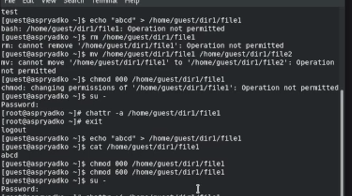
\includegraphics[width=0.6\linewidth,height=\textheight,keepaspectratio]{image/06_remove_a.png}

}

\caption{Успешное изменение файла после снятия защиты}

\end{figure}%
\end{frame}

\begin{frame}[fragile]{Тестирование атрибута \enquote{i} (immutable)}
\phantomsection\label{ux442ux435ux441ux442ux438ux440ux43eux432ux430ux43dux438ux435-ux430ux442ux440ux438ux431ux443ux442ux430-i-immutable}
\begin{itemize}[<+->]
\tightlist
\item
  От имени \texttt{root} установлен атрибут \texttt{i}.
\item
  Данный атрибут делает файл абсолютно неизменяемым: запрещено удаление
  и \textbf{даже дозапись}.
\end{itemize}

\begin{figure}[H]

{\centering 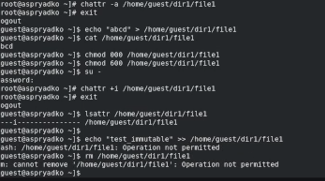
\includegraphics[width=0.6\linewidth,height=\textheight,keepaspectratio]{image/07_attr_i.png}

}

\caption{Полная блокировка файла атрибутом \enquote{i}}

\end{figure}%
\end{frame}

\section{Результаты и
выводы}\label{ux440ux435ux437ux443ux43bux44cux442ux430ux442ux44b-ux438-ux432ux44bux432ux43eux434ux44b}

\begin{frame}[fragile]{Выводы}
\phantomsection\label{ux432ux44bux432ux43eux434ux44b}
\begin{itemize}[<+->]
\tightlist
\item
  Получены практические навыки работы в консоли с расширенными
  атрибутами файлов в ОС Linux.
\item
  Установлено, что атрибут \texttt{a} эффективно защищает файл от
  удаления и перезаписи, оставляя возможность вести логи (дозапись).
\item
  Установлено, что атрибут \texttt{i} делает файл полностью
  \enquote{каменным} (неизменяемым).
\item
  Подтверждено, что управлять политикой расширенных атрибутов может
  исключительно суперпользователь (\texttt{root}).
\end{itemize}
\end{frame}




\end{document}
